\documentclass[../TinyBot.tex]{subfiles}
\begin{document}
    
\section{Motor} \label{sec:motor}
% gearbox, motor

To follow this guide it is not necessary to have an understanding of how motors work,
though it may be interesting for you to learn. The more electrical current passing through
the motor, the more torque the motor is outputting through its shaft. The more torque
the motor outputs, the more it can accelerate. When a load is applied to the motor shaft,
the more current will be needed to continue accelerating. When the load applied to the
motor shaft roughly equals the motor's torque, the shaft stops rotating. This is known
as ``stall torque''. Similarly, ``free current'' is the motor's current draw when the shaft
is rotating without a load. Each motor has its own maximum torque and speed it can output,
which is heavily reliant on the size of the motor. Attempting to go above this limits
can break the motor or overheat the system. \\

This \href{https://www.explainthatstuff.com/electricmotors.html}{link} has a good indepth explanation. 

\bigskip

\subsection{Gear Boxes}

\begin{minipage}[t]{0.6\textwidth}\vspace{0pt}

    Sometimes, we want the motor to output a torque higher than what is can provide.
    Ideally, the motor should be able to output high torques without high currents,
    as the higher the current is the more heat is generated and the more power
    hungry the system is. This can be accomplished with a gearbox.

    Gearboxes can increase torque in exchange for speed or vice-versa. Gearboxes have
    a property called ``gear ratio'' which dictates this change in torque and speed.
    By counting the number of teeth of both the driven and driving gears, the output
    speed and torque can be calculated as below. Notice that $\omega$ is the angular
    speed, $D$ is the diameter, $N$ is the number of teeth, $\tau$ is the torque, and
    $\eta$ is the efficieny (typically ~95\% for a pair of spur gears). Hence, when
    the output gear has more teeth, the torque increases and the speed decreases,
    and vice-versa. Also notice that the driving gear will rotate in the opposite
    direction as the driven gear. \\

\end{minipage}
\begin{minipage}[t]{0.4\textwidth}\vspace{0pt}
    \begin{center}
        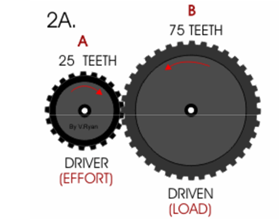
\includegraphics[width=\textwidth]{gear_labelled.png}
        \captionof{figure}{Driver and Driven Gear}
        \label{fig:gear-driver-driven}
    \end{center}
\end{minipage}


\[ R = \frac{N_B}{N_A} = \frac{D_B}{D_A} = \frac{\omega_A}{\omega_B} \]

Hence,

\[ \omega_B = \frac{N_A}{N_B} \cdot \omega_A \]

and

\[ \tau_B = \eta \cdot \frac{N_B}{N_A} \]

When connecting multiple gears, we call this a gear train. There are two types of gear trains:
simple and complex. Simple gear trains are much like their name, simple. They connect next to
each other and you only need to do the calculation for the first gear as an input gear and last
gear as the output gear. These are useful for rapidly increasing torque or speed across a long
distance with a short height. Alternatively, a compound gear train means there can be multiple
gears on the same shaft, meaning the gears on the same shaft will rotate at the same speed and
torque despite being different sizes. You won’t have to deal with compound gear trains for this
project, but feel free to investigate it more. To summarise gears, the ratio of your input gear
to output gear affects the characteristics of your output performance. If you want a higher
torque use a larger output gear. If you want more speed, use a smaller output gear.

\begin{figure}[h]
    \centering
    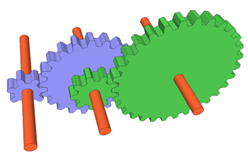
\includegraphics{compound_gears.png}
    \label{fig:gear-complex}
    \caption{Complex Gear Train}
\end{figure}


\end{document}